\documentclass[aip, cp, amsmath, amssymb, reprint, nofootinbib]{revtex4-2}

\usepackage{graphicx}
\usepackage{dcolumn}
\usepackage{bm}

\usepackage{setspace}
\usepackage{graphicx}% Include figure files
\usepackage{fancyhdr}
\setlength{\parindent}{0in}

% Page Formatting
\pagenumbering{arabic} %\pagenumbering{gobble}
\onehalfspacing %doublespacing
\pagestyle{fancy}
%\usepackage{pdfpages}

% Heading Formatting
\headheight 32pt

% Link Formatting
\usepackage{hyperref}
\hypersetup{
	colorlinks,
	allcolors=black
	%citecolor=black,
	%filecolor=black,
	%linkcolor=black,
	%urlcolor=black
}


\usepackage{csvsimple}
\usepackage{mdframed}

\definecolor{commentsColor}{rgb}{0.497495, 0.497587, 0.497464}
\definecolor{keywordsColor}{rgb}{0.541176, 0.168627, 0.886275}
\definecolor{stringColor}{rgb}{0.000000, 0.558215, 0.135316}

% Code Formatting
\usepackage{listings}
\lstset
{ %Formatting for code
	basicstyle=\footnotesize\ttfamily,
	numbers=left,
	%caption={},
	%title={},
	stepnumber=1,
	showstringspaces=false,
	tabsize=1,
	breaklines=true,
	breakatwhitespace=false,
	frame=lines,
	xleftmargin=2em,
	framexleftmargin=1.5em,
	commentstyle=\color{commentsColor}\ttfamily,
  	stringstyle=\color{stringColor}\ttfamily,
	keywordstyle=\color{keywordsColor}\bfseries,
}
\newcommand{\lstprompt}{>\!>\!>}
\newcommand{\numberwithprompt}[1]{\footnotesize\ttfamily\selectfont \lstprompt}


% https://tex.stackexchange.com/questions/340232/how-insert-a-character-at-the-begin-of-every-line-from-a-source-code
\lstdefinestyle{console} {
	basicstyle=\footnotesize\ttfamily,
	numbers=left,
	stepnumber=1,
	showstringspaces=false,
	tabsize=1,
	breaklines=true,
	breakatwhitespace=false,
	frame=single,
	xleftmargin=2em,
	framexleftmargin=2.5em,
	%backgroundcolor=\color{gray!55},
	numberstyle=\numberwithprompt,
	}

% \lstdefinelanguage{psuedocode}{
%   keywords={typeof, new, true, false, catch, function, return, null, catch, switch, var, if, in, while, do, else, case, break},
%   keywordstyle=\color{blue}\bfseries,
%   ndkeywords={class, export, boolean, throw, implements, import, this},
%   ndkeywordstyle=\color{darkgray}\bfseries,
%   identifierstyle=\color{black},
%   sensitive=false,
%   comment=[l]{//},
%   morecomment=[s]{/*}{*/},
%   commentstyle=\color{purple}\ttfamily,
%   stringstyle=\color{red}\ttfamily,
%   morestring=[b]',
%   morestring=[b]"
% }

%\usepackage{algpseudocodex}
%Book Stuff

%\usepackage{algorithm}
%\usepackage[noend]{algpseudocode}
%\makeatletter
%\def\BState{\State\hskip-\ALG@thistlm}
%\makeatother

% Figures & Drawings
\usepackage{graphicx, caption}
\usepackage{animate}
\usepackage{tikz}
\usepackage{float}
\usepackage{pict2e}
\usepackage{subcaption}

% Physics
\usepackage{physics}

% Mathematics
\usepackage{amsmath}
\usepackage{amssymb}
\usepackage{amsthm}
\usepackage{mathtools}
%\usepackage{upgreek} % More Greek letters

% I don't really know what this is but I don't want to break shit
\usepackage{aliascnt}
\newaliascnt{eqfloat}{equation}
\newfloat{eqfloat}{h}{eqflts}
\floatname{eqfloat}{Equation}
\newcommand*{\ORGeqfloat}{}
\let\ORGeqfloat\eqfloat
\def\eqfloat{%
	\let\ORIGINALcaption\caption
	\def\caption{%
		\addtocounter{equation}{-1}%
		\ORIGINALcaption
	}%
	\ORGeqfloat
}
%}

% Bibliography (Citations) Formatting

%\usepackage{cite}
\usepackage{caption}
%\usepackage[backend=bibtex,style=verbose-trad2]{biblatex}
%works really really well, but no MLA format
%\usepackage[backend=biber]{biblatex}
%\bibliographystyle{apsrev4-1}
%\usepackage[backend=biber,style=mla]{biblatex} %Doesn't print all sources for some reason


%\usepackage{graphicx}% Include figure files
\usepackage{dcolumn}% Align table columns on decimal point
\usepackage{bm}% bold math
%\usepackage[mathlines]{lineno}% Enable numbering of text and display math
%\linenumbers\relax % Commence numbering lines

\usepackage[utf8]{inputenc}
\usepackage[T1]{fontenc}
%% Loads a Times-like font. You can also load
%% {newtxtext,newtxtmath}, but not {times}, 
%% {txfonts} nor {mathtpm} as these packages
%% are obsolete and have been known to cause problems.
\usepackage{mathptmx} 


\usepackage{amsthm}
\input{preamble/tikz}
\input{preamble/macros}


% ========================================= %
% LaTeX Template by Aditya K. Rao
% Contact at adi.rao@mail.utoronto.ca

% Change for each document [!!!]
\newcommand\course{PHY426}	% Course Code [!!!]
\newcommand\doctitle{Investigation of Thin Lens Equation and Chromatic Dispersion} % Report Title [!!!]
\newcommand\firstauthorname{Report Author} % Author Name [!!!]
\newcommand\firstauthorstdnum{Student Number: 0000000000} % Student Number [!!!]
\newcommand\firstauthoremail{report.author@mail.utoronto.ca} % Email [!!!]
%\newcommand\secondauthorname{Author Two}
%\newcommand\secondauthorstdnum{Student Number: 0000000000}
%\newcommand\secondauthoremail{report.author@mail.utoronto.ca}
\newcommand\advname{Tahir Shaaran\space} % Advisor Name [!!!]  
\newcommand\taname{Sean Crawford\space} % Advisor Name [!!!] 

\newcommand{\location}{MP222} % Location [!!!]
% ========================================= %
 
% ============== EQUIPMENT ================ %

\newcommand{\oscope}{\texttt{DSOX1202G}\space}
\newcommand{\pdiode}{\texttt{DET36A2}\space}
\newcommand{\hene}{\texttt{HNLS008L}\space}
\newcommand{\cam}{\texttt{Alium 1800 U-500}\space}

% ========================================= %



%\pagenumbering{gobble}
\usepackage{listings}

\renewcommand\lstlistingname{Code Reference}
\renewcommand\lstlistlistingname{Code Reference}
\usepackage{tikz}
\usetikzlibrary{patterns}

\usepackage{circuitikz}

%\addbibresource{references.bib}
\usepackage{lipsum}
\usetikzlibrary{calc}

\begin{document}
\onecolumngrid
\pagenumbering{arabic}
\title{\doctitle}
\author{\firstauthorname}
\email{\firstauthoremail}
\thanks{\firstauthorstdnum}


%\email{report.author@mail.utoronto.ca}
%\thanks{Student Number: 0000000000}
\affiliation{
University of Toronto \\
\location, 60 St. George Street, Toronto, Ontario M5S 1A7, Canada.% Force line breaks with \\ if necessary
}

\date{\today} %Put in date of submission [!!!]

\preprint{APS/123-QED}
\begin{abstract}
    Multiple experiments were conducted to verify the thin lens equation for a variety of different lens types. The focal length of each lens was estimated through two methods. The first being a rudimentary estimation by point source far away and adjusting the lens until a focal point was found. The other by fitting and analyzing the thin lens equation and subsequent modifications. The experiment also characterized the chromatic aberrations in a plano-convex lens under different wavelengths of light. The results of the thin lens experiment were consistent with the theoretical predictions, and the thin lens equation was found to be a good approximation for most of the lenses studied.
\end{abstract}
    \maketitle
    %\tableofcontents 

    \lhead{\firstauthorname\vspace{0.1cm}}
    \chead{\textbf{\course} \\ \doctitle}
    \rhead{\textbf{Prof:} \advname \\ \textbf{TA:} \taname}
    \nocite{*}

    %\newpage
    \twocolumngrid
    \section{Introduction}
        % Plan
        % 1. Relavent Theory
        % 2. Simulation
        % 3. Talk about Hydrogen and Helium Emission Spectra, compare against lens data
        % 4. Talk about relavent theory for that
        % 5. Talk about the setup
        % Data Analysis and Relavent Results, make sure about unceratinties this time

        ptics and lesnes are a cornerstone of modern physics with their applications ranging from the study of the cosmos to the development of modern technology. In this experiment, the thin lens equation was quantiatively verified using a variety of lenses. The experiment was conducted in two parts. The first focused on verifying the thin lens equation, the second investigating if this still holds for thick lenses. Moreover, additional experimentation was conducted to investigate the diffraction patterns of light passing through a lens. Despite their significance, the foundational principles governing optical systems are often taken for granted. This experiment aims to rigorously test the thin lens equation through precise measurements using a variety of lenses.
        
        The experiment is divided into two main parts. The first focuses on verifying the thin lens equation and seeing if it may translate to thick lenses. The second extends this investigation into chromatic abberations in plano-convex lenses under different wavelengths of light.

        \subsection{The Thin \& Thick Lens Equations}
        
        The origins of the thin lens equation have been debated among historians. While the principles of lenses date back to ancient Greece, early mathematical formulations are often attributed to Isaac Barrow (1669) and Christiaan Huygens (1653) \cite{historyoptics}, who provided some of the first semi-verbal descriptions of the equation.
        
        \begin{equation} \label{eqn:thinlens}
            \frac{1}{f} = \frac{1}{p} + \frac{1}{q}
        \end{equation}
        
        Equation \eqref{eqn:thinlens} defines the fundamental relationship between the focal length of a lens ($f$), the object distance ($p$), and the image distance ($q$). A related equation describes the magnification ($M$) of an image.
        
        \begin{equation} \label{eqn:mag}
            M = -\frac{q}{p}
        \end{equation}
        
        Both equations assume that the lens is thin enough to be approximated by a two-dimensional plane rather than a three-dimensional object. In reality, a lens is better represented as having a front principal plane and a back principal plane (\figref{fig:real-lens}).
        
        \begin{figure}[H]
            %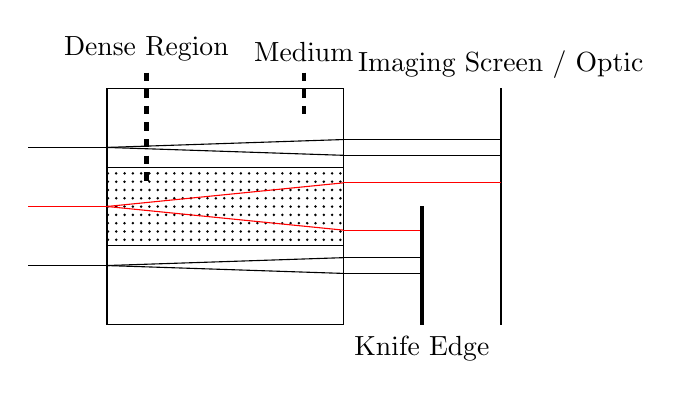
\begin{tikzpicture}
    \def\side{3}
    \def\height{3}
    \def\fmheight{2.5}
    \def\thick{0.25}
    \def\hpthick{0.5}

    \coordinate (TLC) at (-\side/2, \side/2);
    \coordinate (TRC) at (\side/2, \side/2);
    \coordinate (BLC) at (-\side/2, -\side/2);
    \coordinate (BRC) at (\side/2, -\side/2);

    \coordinate (TLC-dense) at ($(TLC)+(0,-1)$);
    \coordinate (TRC-dense) at ($(TRC)+(0,-1)$);
    \coordinate (BLC-dense) at ($(BLC)+(0,1)$);
    \coordinate (BRC-dense) at ($(BRC)+(0,1)$);

    % Draw Medium
    \draw (TLC) rectangle (BRC);

    % Dense Region
    \draw[pattern=dots] (TLC-dense) rectangle (BRC-dense);

    % Parallel Rays
    \draw ($(TLC)+(-1,-\side/4)$) -- ($(TLC)+(0,-\side/4)$);
    \draw[color=red] ($(TLC)+(-1,-\side/2)$) -- ($(TLC)+(0,-\side/2)$);
    \draw ($(TLC)+(-1,-3*\side/4)$) -- ($(TLC)+(0,-3*\side/4)$);

    % Refracting Rays
    \draw ($(TLC)+(0,-\side/4)$) -- ($(TRC)+(0,-\side/4+0.1)$);
    \draw[color=red] ($(TLC)+(0,-\side/2)$) -- ($(TRC)+(0,-\side/2+0.3)$);
    \draw ($(TLC)+(0,-3*\side/4)$) -- ($(TRC)+(0,-3*\side/4+0.1)$);

    % Refracting Rays
    \draw[color=black] ($(TLC)+(0,-\side/4)$) -- ($(TRC)+(0,-\side/4-0.1)$);
    \draw[color=red] ($(TLC)+(0,-\side/2)$) -- ($(TRC)+(0,-\side/2-0.3)$);
    \draw[color=black] ($(TLC)+(0,-3*\side/4)$) -- ($(TRC)+(0,-3*\side/4-0.1)$);

    % Refracted Rays
    \draw ($(TRC)+(0,-\side/4+0.1)$) -- ($(TRC)+(1,-\side/4+0.1)$);
    \draw[color=red] ($(TRC)+(0,-\side/2+0.3)$) -- ($(TRC)+(1,-\side/2+0.3)$);
    \draw ($(TRC)+(0,-3*\side/4+0.1)$) -- ($(TRC)+(1,-3*\side/4+0.1)$);
    
    % Refracted Rays
    \draw[color=black] ($(TRC)+(0,-\side/4-0.1)$) -- ($(TRC)+(1,-\side/4-0.1)$);
    \draw[color=red] ($(TRC)+(0,-\side/2-0.3)$) -- ($(TRC)+(1,-\side/2-0.3)$);
    \draw[color=black] ($(TRC)+(0,-3*\side/4-0.1)$) -- ($(TRC)+(1,-3*\side/4-0.1)$);

    % Knife Edge
    \coordinate (ket) at ($(TRC)+(1,0)$);
    \coordinate (kec) at ($(TRC)+(1,-\side/2)$);
    \coordinate (keb) at ($(BRC)+(1,0)$);

    \draw[ultra thick] (kec) -- (keb)node[anchor=north]{Knife Edge};

    
    % Screen
    \coordinate (scc) at ($(TRC)+(2,-\side/2)$);
    \coordinate (sct) at ($(TRC)+(2,0)$);
    \coordinate (scb) at ($(BRC)+(2,0)$);

    \draw[thick] (sct)node[anchor=south]{Imaging Screen / Optic} -- (scb);

    % Post Knife Edge Ray
    \draw ($(ket)+(0,-\side/4+0.1)$) -- ($(sct)+(0,-\side/4+0.1)$);
    \draw ($(ket)+(0,-\side/4-0.1)$) -- ($(sct)+(0,-\side/4-0.1)$);
    \draw[color=red] ($(ket)+(0,-\side/2+0.3)$) -- ($(sct)+(0,-\side/2+0.3)$);

    % Medium Label
    \draw[ultra thick, dashed] ($(TLC)+(2*\side/3+0.5,0.2)$)node[anchor=south]{Medium} -- ($(TLC)+(2*\side/3+0.5,-0.4)$);

    \draw[ultra thick, dashed] ($(TLC)+(\side/3-0.5,0.2)$)node[anchor=south]{Dense Region} -- ($(TLC)+(\side/3-0.5,-1.2)$);

\end{tikzpicture}
            \includegraphics[width=0.8\linewidth]{figures/fp-bp.png}
            \caption{Illustration of principal planes in a real (thick) lens, adapted from the laboratory manual \cite{labmanual}.}
            \label{fig:real-lens}
        \end{figure}
        
        As can be seen in \figref{fig:real-lens}, there is indeed some ofset between the front and back principal planes. This offset is crucial in determining the focal length of a thick lens where this difference is exacerbated. Therefore, one may us \eqref{eqm:thicklens} to obtain a better approximation of the focal length of a thick lens.

        \begin{equation} \label{eqm:thicklens}
            \frac{1}{f} = \frac{1}{|o-l|-p_f} + \frac{1}{|i-l|-p_b}
        \end{equation}
        
        Where $p_f$ and $p_b$ are the distances from the front and back principal planes to the object and image respectively. $p = |o-l|$ and $q = |i-l|$ are the distances from the object and image to the lens respectively. Then,  thin lens equation is just a special case of \eqref{eqm:thicklens} with $p_f = p_b = 0$.

        \subsection{Chromatic Aberrations}
        
        Lenses in practical applications rarely behave as ideal thin lenses due to inherent optical imperfections. These deviations, known as aberrations, can significantly affect image quality. In general, there are five primary Seidel aberrations including \textit{spherical aberration}, \textit{coma}, \textit{astigmatism}, \textit{field curvature}, and \textit{distortion}. These aberrations can be further classified into two categories: geometric and chromatic. Additional study was specifically conducted \textit{chromatic aberrations}, or coma, which occur as a result of light dispersion within the optical matieral of the lens. The dispersion relation for a dielectric material is given in \eqref{eqn:dispersion}.

        \begin{equation} \label{eqn:dispersion}
            n^2(\omega) = 1 + \frac{N^2}{\varepsilon_0 m _e}\frac{1}{\omega_0^2 - \omega^2}
        \end{equation}

        Which may further be reduced \cite{labmanual} to \eqref{eqn:dispersion2} to solve for $\omega$.

        \begin{equation} \label{eqn:dispersion2}
            \frac{1}{n^2 - 1} = \frac{C}{\lambda_c^2} - \frac{C}{\lambda^2} 
        \end{equation}

        Where $C$ and $\lambda_c$ are constants for the material and $\lambda$ is the wavelength of the light, and $n$ is the refractive index. For air, this may be calculated using the len's maker equation \eqref{eqn:lensmaker}.

        \begin{equation} \label{eqn:lensmaker}
            \frac{1}{f} = (n-1)\left[\frac{1}{R_1} - \frac{1}{R_2} + \frac{(n-1)d}{n R_1 R_2}\right]
        \end{equation}

        WHere $R_1$ and $R_2$ are the radii of curvature of the lens and $d$ is the thickness of the lens. 

        Specifically, for this section of the experiment, the change in the focal length of a plano-convex lens was measured under different wavelengths of light (i.e. different colors). These results were compared to a known wavelength as calculatd by a triprism spectroscope with calibration equation given in \eqref{eqn:triprism}.

        \begin{equation} \label{eqn:triprism}
            y = \frac{m}{\lambda-\lambda_0} + b
        \end{equation}

        Where $\lambda_0$ is predeterimned for each spectroscope.


    \section{Methodology}

        The experiment was conducted using a $1.500\pm0.005\,\text{m}$ optical bench equipped with a light source, diaphragms, lenses, and a screen. The apparatus was arranged as in \figref{fig:expsetup}. The distances between optical elements were recorded using the built-in ruler of the optical bench. To account for systematic errors, offsets between the mount edges and the optical centers of the elements were measured using calipers with a precision of $\pm0.1\,\text{mm}$. Uncertainties in these measurements were estimated by taking the statistical uncertainty of multiple readings.

        \begin{figure}[H]
            \centering
            %\input{figures/expsetup.tex}
            \includegraphics[width=0.8\linewidth]{figures/optical-bench.png}
            \caption{Experimental setup for measuring the focal length of a lens. This image specifically looks how how measurements wer taken using reference lengths.}
            \label{fig:expsetup}
        \end{figure}

        Proper alignment of the optical components was critical. Three primary components were used:, a light source\footnote{Exact model number and manufacturer to be recorded.}, a variable diaphram apperature, a lens mounted on vertical and horizontal translation stage, and a screen. Adjustments were first made near to the point light source to ensure the beam was aligned correctly. The screen was then progressively moved back until the image remained at the same inital point on the screen. Fine adjustments were initially made on the lamp's translation and adjustment stages with later adjustments being made on the lens mount.

        Onece a lens was placed within the mount, the lens was adjusted vertically and horizontally using translation stages until the backreflection of the lens was directly back into the bulb.

        \begin{figure}[H]
            \centering
            %\input{figures/far-field.tex}
            \includegraphics[width=0.8\linewidth]{figures/setup.jpeg}
            \caption{Actual experimental setup used. The lamp is positioned at the edge of the optical rail on a horizontal translation stage. Additional adjustments could be made to the bulb, though this significantly affected alignment and was difficult to tune.}
            \label{fig:realsetup}
        \end{figure}

        % Alignment Procedures  
        Initial estimates of the focal length of each lens were obtained using a far field method. The lens was placed at a distance from the light source such that the image formed was at the far field. The distance between the lens and the screen was then measured to obtain the focal length. This method was repeated for each lens to ensure consistency.
        % \begin{enumerate}
        %     \item The lamp was positioned behind a diaphragm with a small aperture to produce a collimated beam.
        %     \item A screen was placed at a short distance from the diaphragm to check for alignment by marking the central light spot.
        %     \item The lens was positioned approximately 7 cm from the diaphragm, and its angle was adjusted to retro-reflect light back through the aperture.
        %     \item The screen was moved about 1 m away to observe the far-field focus, ensuring the beam remained centered.
        %     \item Fine adjustments were made iteratively to confirm proper alignment.
        % \end{enumerate}

        An additional grid was placed before the lens to measure geometric magnification and any distortions introduced by the lens. Given there was some distortion despite multiple realignment attempts, a $3\times3$ unit block of values was recorded as well as multiple readings for each configuration.

        \begin{figure}[H]
            \centering
            %\input{figures/far-field.tex}
            \includegraphics[width=0.8\linewidth]{figures/grid.jpeg}
            \caption{$3\times3$ grid points used to mitigate distorition effects present.}
            \label{fig:grid}
        \end{figure}

        % \subsection{Focal Length Estimation}
        % The focal length of each lens was estimated through two methods:
        % \begin{enumerate}
        %     \item Measuring the image distance when the lens was far from the light source.
        %     \item Using the lensmaker's equation:
        %     \begin{equation}
        %         f = \frac{R}{2(n-1)}
        %     \end{equation}
        %     where $R$ is the radius of curvature and $n$ is the refractive index of the lens material.
        % \end{enumerate}

        For data collection post alignment, the position of the source was fixed for all measurements. The lens was then placed at $5$ different locations on the optical bench. At each location, $3$ measurements were taken by moving the screen to obtain a sharp image of the grid, this image distance was then recorded. This procedure was repeated for a variety of lenses, namely a plano-convex lens, a biconvex lens, a concave-convex lens, and a spherical lens. 
        
        The magnification was calculated by measuring the grid line spacing in the image. The process was repeated for a range of object and image distances. Data was verified by checking consistency with \eqref{eqn:thinlens}.

        For thicker lenses, additional measurements were taken to determine whether the thin lens approximation remained valid. The locations of the front and back principal planes were estimated, and deviations from the ideal thin lens behavior were analyzed.



    \section{Results \& Analysis}
        \subsection{Thin Lens Investigation}
            \textcolor{red}{\textbf{[Include new graphs and analysis for thin lens investigation.]}}

            \begin{figure}[H]
                \centering
                %\input{figures/thin-lens.tex}
                \includegraphics[width=0.9\linewidth]{figures/ideallens.png}
                \caption{Focal length of a plano-convex lens as a function of object distance.}
                \label{fig:thin-lens}
            \end{figure}

            % \begin{figure}[H]
            %     \centering
            %     %\input{figures/thick-lens.tex}
            %     \includegraphics[width=0.9\linewidth]{figures/thicklens.png}
            %     \caption{Focal length of a thick lens as a function of object distance.}
            %     \label{fig:thick-lens}
            % \end{figure}


        \subsection{Thick Lens Investigation}
            \textcolor{red}{\textbf{[Include new graphs and analysis for thin lens investigation.]}}        

        \subsection{Chromatic Aberrations}

            Data points taken for triprism calibration are shown in \figref{fig:chromatic-He} and \figref{fig:chromatic-H}. These were both fit to \eqref{eqn:triprism} to obtain the calibration constants. The spectroscope constant was provided $\lambda_0 = 284.6 \pm 0.4\,\text{nm}$.

            \begin{figure}[H]
                \centering
                %\input{figures/chromatic.tex}
                \includegraphics[width=0.9\linewidth]{figures/spec-he.png}
                \caption{Calibration curve for the triprism spectroscope using a $\text{He}$ sample. Fit parameters $m = 1000\pm700$, $\b=-9\pm 1$, $\chi^2_{\text{red}} = 1248$. Residuals show some pattern indicating an under estimation of uncertainties.}
                \label{fig:chromatic-He}
            \end{figure}


            \begin{figure}[H]
                \centering
                \includegraphics[width=0.9\linewidth]{figures/spec-he.png}
                \caption{Calibration curve for the triprism spectroscope.}
                \label{fig:chromatic-H}
                \caption{Calibration curve for the triprism spectroscope using a $\text{H}$ sample. Fit parameters $m = 500\pm100$, $\b=-0.3\pm 2$, $\chi^2_{\text{red}} = 230$. Residuals show some pattern indicating an under estimation of uncertainties.}
                \label{fig:chromatic-H}
            \end{figure}

            Clearly, both fits show some pattern in the residuals indicating that the uncertainties were underestimated. However, qualitatively, this fits do indeed look decent. However, it should be noted that some odd observations were observed during data collection. Namely, multiple additional spectral lines were visable in both the $\text{He}$ and $\text{H}$ samples\footnote{This phenomena was also observed by the technical staff}. However, this did not significantly affect the results of the experiment. 

            \textcolor{red}{\textbf{[Include application for green and red absorbing filters.]}}

    
    \section{Conclusion}
        This study effectively quantitatively verified the thin lens equation for most of the lenses studied. The experimental setup consisted of an optical rail/bench with a lamp, adjustable iris apperature, lens holder on vertical (and horizontal) translation stage, and a screen. Uncertainties were estimated using both statistical and systematic methods. with the later being from the gradations on measurement tools and the former being from the standard deviation of multiple readings.
        
        Additional measurements were taken to characterize the chromatic aberrations in a plano-convex lens. The focal length of the lens was measured under different wavelengths of light, and the results were compared to a known wavelength. \textcolor{red}{[Include results of chromatic aberrations]}.


        It was found that, for the most part, the thin lens equation held true for the lenses studied. However, for the thicker lenses, the thin lens approximation was not as accurate. This was expected as the thin lens equation is a simplification of the more general thick lens equation. The focal length of the lenses was measured using a variety of methods, including the far field method and the lensmaker's equation. The magnification was also calculated by measuring the grid line spacing in the image. \textcolor{red}{[Include numerical results from new analysis]}.


    % Line to seperate report content from acknowledgements and references
\onecolumngrid
\begin{center}
    \vspace{0.8cm}
    \noindent\rule{0.9\textwidth}{0.5pt}
\end{center}

\begin{acknowledgments}
    The author would like to thank Prof. \advname (Supervising Professor) and \taname (Teaching Assistant) for their guidence and support throughout the experiment. Moreover, the author would like to further acknowledge the support of the lab technician team L. Avramidis and P. Scolieri for their assistance in debugging issues that arose with the triprism spectroscope. Finally, the support of author experimentors in MP250 should be acknowledged as they provided valuable feedback and suggestions during the experiment.
\end{acknowledgments}

\bibliography{references}

% \appendix
% \section{Appendix}

% \subsection{Raw Data}

% \subsection{Code}

\end{document}